% --------------------------------------------------------------------
% LaTeX Template for Math Worksheets
% --------------------------------------------------------------------
\documentclass{article}

% --- PACKAGE IMPORTS ---
% These packages add functionality for math symbols, formatting, etc.
\usepackage[margin=.7in]{geometry}       % For setting page margins to 0.7 inch
\usepackage{amsmath, amssymb, amsthm}   % American Mathematical Society packages for advanced math
\usepackage{graphicx}                   % For including images
\usepackage{fancyhdr}                   % For creating custom headers and footers
\usepackage[colorlinks=true, urlcolor=blue, linkcolor=blue]{hyperref} % For clickable links
\usepackage{cancel}
\usepackage{array}
\usepackage{amsfonts}
\usepackage{amsxtra}
\usepackage{epsfig}
\usepackage{wasysym}
\usepackage{relsize}
\usepackage{tikz}
\tikzset{every picture/.style={scale=1.2}}
\usetikzlibrary{decorations.markings} 
\renewcommand{\normalsize}{\fontsize{12}{20}\selectfont}

% custom commands
\newcommand{\myauthor}{Miguel Gomez}
\newcommand{\canceling}[2]{\textcolor{red}{\cancelto{\textcolor{black}{#1}}{\textcolor{black}{#2}}}}
\newcommand{\todo}[1]{\textcolor{blue}{TODO:#1}}
% Save the original commands
\let\oldcos\cos
\let\oldsin\sin
\let\oldcosh\cosh
\let\oldsinh\sinh

% Redefine with automatic parentheses
\renewcommand{\cos}[1]{\oldcos\left(#1\right)}
\renewcommand{\sin}[1]{\oldsin\left(#1\right)}
\renewcommand{\cosh}[1]{\oldcosh\left(#1\right)}
\renewcommand{\sinh}[1]{\oldsinh\left(#1\right)}

\newcommand{\der}[2]{\frac{d#1}{d#2}}
\newcommand{\secder}[2]{\frac{d^2#1}{d#2^2}}
\newcommand{\parder}[2]{\frac{\partial#1}{\partial#2}}
\newcommand{\secparder}[2]{\frac{\partial^2#1}{\partial#2^2}}

% --- DOCUMENT & AUTHOR INFORMATION ---
\title{Worksheet \# 9}
\author{
  MATH 3160 -- Complex Variables\\
  \myauthor
}
\date{Completed: \today} 

% --- HEADER & FOOTER CONFIGURATION ---
% This section sets up the header that will appear on each page.
\pagestyle{fancy}
\fancyhf{} % Clears the default header and footer
\lhead{Math 3160 -- Worksheet \# 9} % Left side of header
\rhead{\myauthor} % Puts the author's name on the right side
\rfoot{Page \thepage} % Puts the page number on the bottom right

\begin{document}

\maketitle % This command generates the title based on the information above.

% ====================================================================
% --- START OF PROBLEMS ---
% ====================================================================

% Note: \section* creates a section heading without a number.
\section*{Problem 1}
let C be the contour shown below, traversed counter-clockwise from the blue point to the red. I have reconstructed this image from the worksheet and am confident this is similar to how it was done, but I must admit I am making an assumption about the structure. 
\begin{center}
\begin{tikzpicture}
    % Draw grid
    \draw[gray!30, very thin] (-2.5,-2.5) grid (2.5,2.5);
    
    % Draw axes
    \draw[->] (-2.5,0) -- (2.5,0) node[right] {};
    \draw[->] (0,-2.5) -- (0,2.5) node[above] {};
    
    % Add axis labels
    \foreach \x in {-2,-1,1,2}
        \draw (\x,0.1) -- (\x,-0.1) node[below] {\x};
    \foreach \y in {-2,-1,1,2}
        \draw (0.1,\y) -- (-0.1,\y) node[left] {\y};
    
    % Draw the wavy circle with arrow decorations
    \draw[thick] plot[domain=-225:45, samples=300, smooth] 
        ({\x}: {sqrt(2) + 0.05*sin(40*\x)});
        % Draw the wavy circle with arrow decorations
    \draw[gray!30, decoration={markings, 
        mark=at position 0.15 with {\arrow[black]{>}},
        mark=at position 0.35 with {\arrow[black]{>}},
        mark=at position 0.55 with {\arrow[black]{>}},
        mark=at position 0.75 with {\arrow[black]{>}},
        mark=at position 0.95 with {\arrow[black]{>}}},
        postaction={decorate}] 
        plot[domain=-225:45, samples=300, smooth] 
        ({\x}: {sqrt(2.8)});


    % Add dots at start and end points
    \fill[red] (45:{sqrt(2)}) circle (2pt);
    \fill[blue] (-225:{sqrt(2)}) circle (2pt);
\end{tikzpicture}
\end{center}
\vspace{0.5cm} % Add space for additional work if needed

% steal fig from the latex given on canvas

find $\int_C \frac{1}{z}dz$ (Hint: Consider a new branch of the logarithm function by $\log{(re^{i\theta})} = \ln{(r)} + i\theta$, where $-3\pi/2 < \theta \leq \pi/2$, and check that this is an anti-derivative of $1/z$.)
\vspace{0.5cm}
\hrule % Adds a horizontal line to separate problems.
\vspace{0.5cm}
I get the hint, but I saw this from the start and wanted to work it out. In checking this path, we know that the result should have a value because it is not a closed path. Parametrizing this path works as follows given the diagram. placing a circle of radius $\sqrt{2}$ cuts through the sinusoid and it oscillates around it.  
\begin{align*}
  z &= (\sqrt{2}+A\sin{\omega\theta})e^{i\theta} \\
  z_0 &= \sqrt{2}e^{-i\frac{5\pi}{4}} \quad A\sin{-\omega\frac{5\pi}{4}} = 0 \\
  z_f &= \sqrt{2}e^{i\frac{\pi}{4}}  \quad A\sin{\omega\frac{\pi}{4}} = 0\\
  r(t) &= \sqrt{2}+A\sin{\omega\theta(t)}
\end{align*}

The path has a sinusoidal signal in superposition such that there is a change $A\sin{\omega\theta}$ in the magnitude of $z$. Instead of writing out so much, we can continue by treating this more generally:

\begin{align*}
  z(t) &= r(t)e^{i\theta(t)} \\
  z'(t) &= r'(t)e^{i\theta(t)}+r(t)(i\theta'(t))e^{i\theta(t)}\\
  \int_{\gamma}f(z)dz &= \int_{t_0}^{t_1}f(z(t))z'(t)dt \\
  \int_{\gamma}f(z)dz &= \int_{t_0}^{t_1}\frac{1}{r(t)e^{i\theta(t)}}[r'(t)e^{i\theta(t)}+r(t)(i\theta'(t))e^{i\theta(t)}]dt \\
&= \int_{t_0}^{t_1}\frac{e^{i\theta(t)}}{r(t)e^{i\theta(t)}}[r'(t)+r(t)(i\theta'(t))]dt \\
       &= \int_{t_0}^{t_1}\left[\frac{r'(t)}{r(t)}+i\theta'(t)\right]dt \\
  &= \int_{t_0}^{t_1}\frac{r'(t)}{r(t)}dt +i\int_{t_0}^{t_1} \theta'(t)dt \\
  &= \ln{(r(t))}|_{t_0}^{t_1} +i \theta(t)|_{t_0}^{t_1} \\
  &= (\ln{(r(t_1))} - \ln{(r(t_0))}) + i (\theta(t_1)-\theta(t_0)) \\
\end{align*}
Now, we can see that no matter the function $r(t)$, we get the final expressions by recognizing that the  sinusoidal signal for the magnitude has the same value at $t_0$ and $t_1$, then $r(t_1) = r(t_0)$, and therefore $\ln{(r(t_1))} = \ln{(r(t_0))}$. This then leaves us with the final expression:
\begin{align*}
\int_{\gamma}f(z)dz &=  i (\theta(t_1)-\theta(t_0))
\end{align*}
This shows that the integral value only depends on the angle difference and would not change for any radius used. Therefore, since the angular difference is $3/4$ of the unit circle, and we know the integral of $1/z$ is $2\pi i$, this integral is therefore $\frac{3\pi}{2} i$. Which is nice because it confirms the given hint and why it works as an antiderivative.
\newpage
\section*{Problem 2}
Show that $\int_C f(z)dz = 0$ for $C$ the unit circle and :
\begin{enumerate}
  \item[(i)] $f(z) = \frac{z^2}{z+3}$
  \item[(ii)] $f(z) = \frac{1}{z^2 + 2z + 2}$
\end{enumerate}
\subsection*{(i)}
Since we are evaluating with $C$ within the unit circle, any point which lies outside of the unit circle does not matter for our evaluation as we only need the curve and its interior to be a simply connected domain $D$. in the denominator, we see that we have $z+3$, meaning that it only becomes 0 if $z$ is $-3$. So the point $z = -3$ in the complex plane will give a divide by zero issue. Since $|−3| = 3 > 1$, the unit circle only contains points where the magnitude of $z$ is less than or equal to $1$, meaning it is analytic inside and on the unit circle.

$\therefore$ the C-G theorem holds and we have a path with a simply connected interior region with the same starting and ending point whose integral evaluates to $0$. 

\subsection*{(ii)}
In this problem, we have a similar result as the denominator is $0$ only where $z = -1 \pm i$ given the factoring of the denominator. Notice that the magnitude of $z$ for these points will be $\sqrt{2}$, and therefore the points are also outside of the unit circle. With $\sqrt{2} > 1$ and the unit circle only contains points where $|z| \leq 1$, then we again have an integral that evaluates to $0$. 

\vspace{0.5cm} % Space for work

\hrule

\newpage
\section*{Problem 3}
Let $C_1$ denote the positively oriented boundary of the square whose sides lie along the lines $x = \pm 1$, and $y=\pm i$, and let $C_2$ denote the positively oriented circle $|z| = 4$. Explain why:
\begin{align*}
  \int_{C_1}f(z)dz &= \int_{C_2}f(z)dz
\end{align*}
when
\begin{enumerate}
  \item[(a)] $f(z) = \frac{1}{3z^2+1}$
  \item[(b)] $f(z) = \frac{z+2}{sin(z/2)}$
  \item[(c)] $f(z) = \frac{z}{1-e^z}$
\end{enumerate}

\vspace{0.5cm} % Space for work

\hrule

\begin{center}
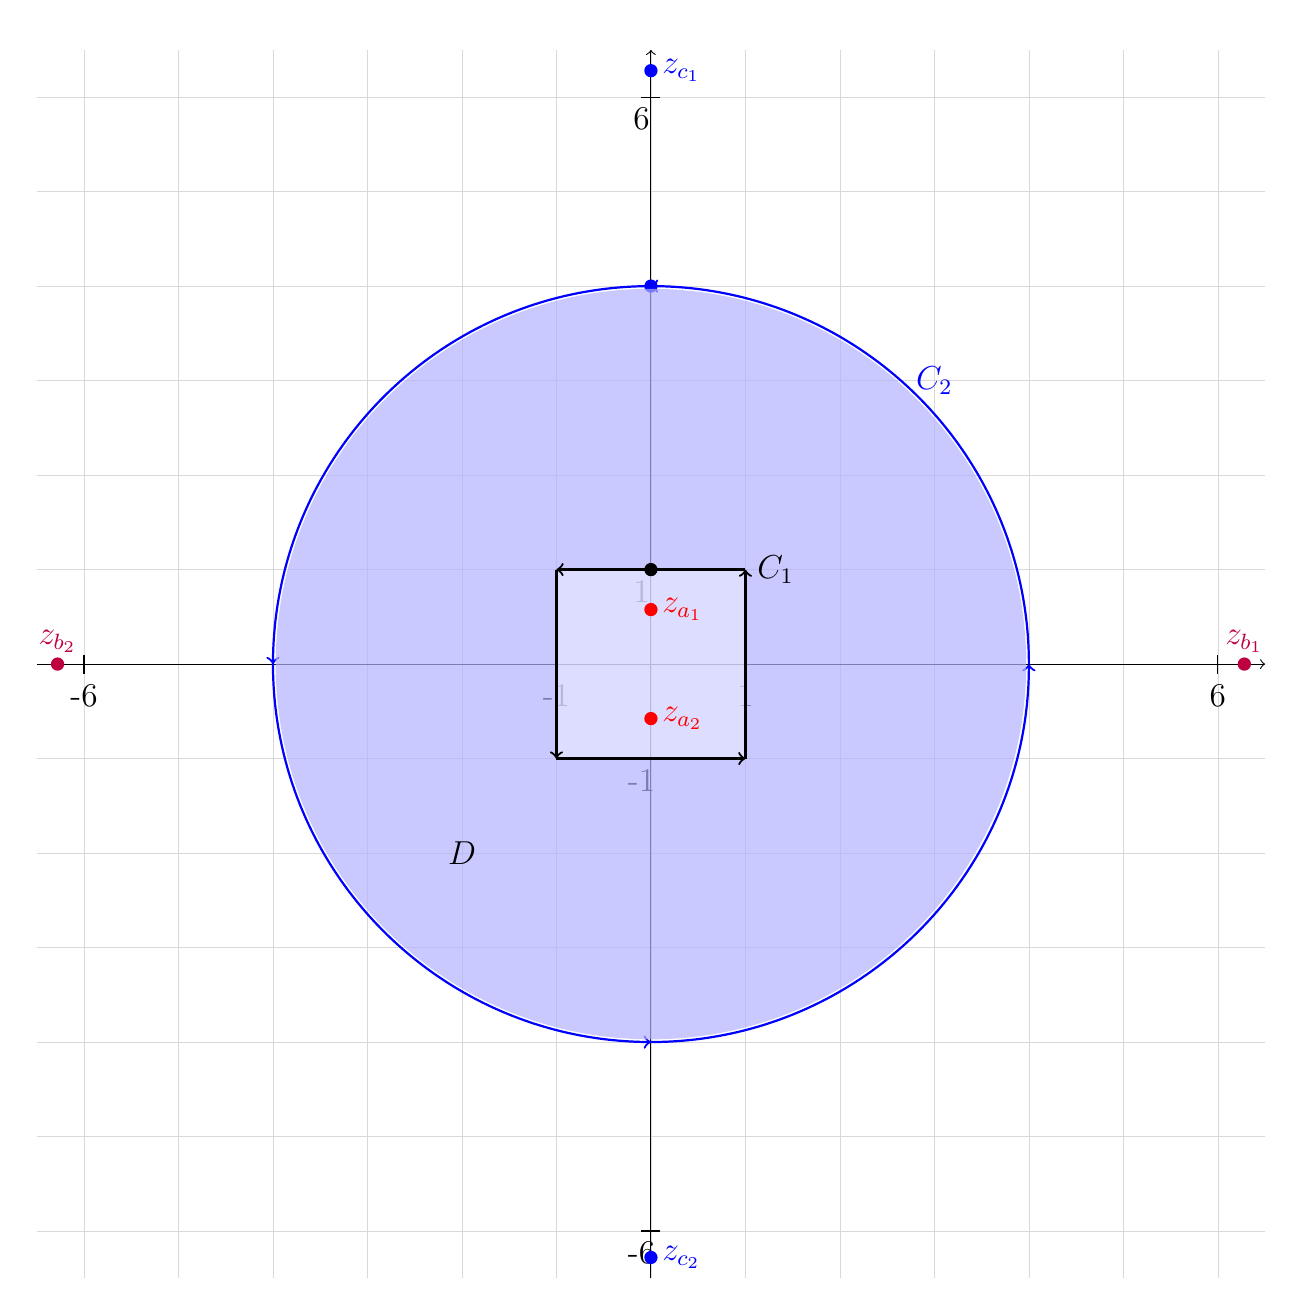
\begin{tikzpicture}
    % Draw grid
    \draw[gray!30, very thin] (-6.5,-6.5) grid (6.5,6.5);
    
    % Draw axes
    \draw[->] (-6.5,0) -- (6.5,0) node[right] {};
    \draw[->] (0,-6.5) -- (0,6.5) node[above] {};
    
    % Add axis labels
    \foreach \x in {-6,-1,1,6}
        \draw (\x,0.1) -- (\x,-0.1) node[below] {\x};
    \foreach \y in {-6,-1,1,6}
        \draw (0.1,\y) -- (-0.1,\y) node[below] {\y};
    
    % Add dots at start and end points
    \fill[blue] (0,4) circle (2pt);
    \draw[blue, ->, decoration={markings, 
        mark=at position 0.25 with {\arrow{>}},
        mark=at position 0.5 with {\arrow{>}},
        mark=at position 0.75 with {\arrow{>}}},
      postaction={decorate}, thick] (4,0) arc (0:360:4);
      \draw[blue] (3, 3) node[] {$C_2$};
\fill[blue!30, opacity=0.7] (0,0) circle (113pt);
\fill[blue!05, opacity=0.5] (-1,-1) rectangle (1,1);        
        \fill[black] (0,1) circle (2pt);
    \draw[thick, black, ->] (1,1) -- (-1,1);
    \draw[thick, black, ->] (-1,1) -- (-1,-1);
    \draw[thick, black, ->] (-1,-1) -- (1,-1);
    \draw[thick, black, ->] (1,-1) -- (1,1) node[right] {$C_1$};    
      \draw[Black] (-2, -2) node[] {$D$};

      \fill[red] (0,.577) circle (2pt) node[right] {$z_{a_{1}}$};
      \fill[red] (0,-.577) circle (2pt) node[right] {$z_{a_{2}}$};

      \fill[purple] (6.28, 0) circle (2pt) node[above] {$z_{b_{1}}$};
      \fill[purple] (-6.28, 0) circle (2pt) node[above] {$z_{b_{2}}$};

      \fill[blue] (0, 6.28) circle (2pt) node[right] {$z_{c_{1}}$};
      \fill[blue] (0, -6.28) circle (2pt) node[right] {$z_{c_{2}}$};
      
\end{tikzpicture}
\end{center}

\subsection*{(a)}
The poles for the expression $\frac{1}{3z^2 + 1}$ lie within the region defined by $C_1$ as shown in the figure as $D$ in the darker blue shaded region minus the interior. Since we are evaluating things within the region bound by $C_1$ and $C_2$, we can use Cauchy's theorem to evaluate. The theorem states an analytic function on a domain $D$ and its boundary resolves in 0. Since the expression is analytic on the boundaries and the region, then we know the two integrals will evaluate to 0, making the overall expression, with the two integrals on the boundaries being equal, true.

i.e.
\begin{align*}
  \int_{C_1}f(z)dz &- \int_{C_2}f(z)dz = 0 \\
  \int_{C_1}f(z)dz &= \int_{C_2}f(z)dz
\end{align*}

\subsection*{(b)}
Similarly here, the poles for this expression lie on complex number values of $z/2 = n\pi$ which are values of $2n\pi$. Looking at the first few values:
\begin{align*}
  z = \{0, \pm 2\pi, \pm 4\pi, ...\}
\end{align*}
The first two of these are pictured in the figure and lie within the first boundary being $0$, and the outside due to $|4| < |\pm 2\pi|$. Since the poles lie outside the domain $D$, same as in $(a)$, we can see that Cauchy's theorem again holds true as $f$ is analytic on the boundaries and the domain $D$. 
\subsection*{(c)}
This expression has poles only when $1-e^z = 0$ which happens when $z = n2\pi i$. These too are pictured on the figure. These show the same situation as $(b)$, with the poles rotated by $90\circ$ as we would expect with the extra factor of $i$. In the same fashion as $(b)$, the poles lie outside the circle of radius $4$, making Cauchy's theorem apply and we can evaluate the integrals over the domain $D$ and along their boundaries, making the overall equality true.  

\end{document}

%%% Local Variables:
%%% mode: latex
%%% TeX-master: t
%%% End:
